%!TEX root = ../BoYu-Dissertation.tex
\graphicspath{{Figures/}}

\chapter{Our Approach: Modeling the Filed of Work} % (fold)
\label{cha:field_of_work}

We employ the computational theory of SharedPlan \cite{grosz1996collaborative,Grosz98theevolution} to represent collaborative activities as shared plans, and then use this model of activities to derive the knowledge about local scopes of work and dependencies. In the following parts of this chapter, we first describe the basis and different components of the SharedPlan model, then describe how the different components of the filed work can be represented using the PlanGraph model.

\section{Formalizing the Field of Work in SharedPlan Theory}
Rooted in the SharedPlans theory \cite{grosz1996collaborative,Grosz98theevolution}, the proposed activity model treats a collaborative activity as an evolving shared plan situated in a set of physical and mental contextual factors. In general, a shared plan is a moment-to-moment representation of an unfolding activity and includes not only a hierarchy of actions but also the set of mental states (beliefs, intentions, and commitments) that the participating actor have established towards the activity, and the knowledge preconditions and physical constraints that have to be satisfied prior to an activity being performed.

\subsection {SharedPlan Theory}
\subsubsection*{Action Decomposition}
The SharedPlans theory models an activity as hierarchically structured subsidiary actions that are intended and performed in some specific context components. An \textbf{action} refers to a specific goal as well as the effort needed to achieve it. An action can be either basic or complex. A \emph{basic} action can be directly executed by one or multiple actors. A \emph{complex} action, however, cannot be directly executable because it needs to be decomposed into subsidiary actions. The concept of action in SharedPlan theory has a broad definition, which includes the high-level collaborative activity, the medium-level actions, and the low-level operations.

The knowledge preconditions are called \textbf{parameters} of the action that have to be identified prior to an action being performed, i.e. actors must be able to identify the parameters of the action to be performed. A parameter can represent the knowledge about an object of the action or a resource used by the action. It is shared and visible to the action it belongs to and all the sub-actions. If a parameter has not been identified, the actors need to develop a plan to identify the parameter before the action can be performed.

A \textbf{precondition} defines a certain proposition that indicates certain states of a parameter or relationships among multiple parameters must be satisfied in order to perform an action. As a result, any variables in a precondition must also appear in the action's parameter list. 

\subsubsection*{Mental States}
The SharedPlans theory provides a formal specification of the mental attitudes requirements of participants in a collaborative activity. The specification is given in terms of beliefs, mutual beliefs, and intentions of the participants. It deploys two intentional attitudes, intending to (do an action) and intending that (a proposition hold). Intentions-to are used to represent an agent’s commitments to its own actions. Such commitments instigate means-end reasoning about ways of accomplishing its intended actions – that is, to planning. Intentions-that are used to represent an agent’s commitments toward a joint activity and the actions of its fellow participants in service of that activity. Such commitments lead an agent to engage in reasoning about other participant’s actions and intentions and ways the agent could contribute to their success in the context of the group activity. Besides, an indicator of the current attentional state, representing whether an action is the current focus of an actor is also included. 

\subsubsection*{Partiality of Plans}
A critical point made in the SharedPlans theory is that planning is interleaved with acting, which means agents can act on partial recipes, and a group of agents may not have a complete plan until after they have done some of the actions in the partial recipe. To have a partial shared plan means there are still some actions that remain to be resolved (i.e., role assignment) or decomposed further. In the beginning of the collaboration, the agents only have a partial shared plan of the activity, which merely consists of the agent’s initial intention of performing the activity. With the development of the activity, the agents collaboratively elaborate the activity by selecting recipe for it, breaking it down into subsidiary actions, and updating their beliefs and intentions towards these subsidiary actions. In this course, the shared plan evolves and when it reaches the status of a full shared plan, the collaboration ends up with the underlying activity successfully performed.

The SharedPlans theory has the benefits to address the aforementioned challenges of modeling an activity:  (1) the internal mental states of the user are modeled as the intentions, beliefs, and mutual beliefs of the participants; (2) the activity is modeled as hierarchically structured actions that are intended and performed in some specific context components (e.g. constrains, knowledge preconditions, intentional structure, and attentional state etc.); (3) the development of an activity is modeled as the evolution from a partial shared plan to a full one. 

A plan of an action is a description of the action in the specific collaborative context. The difference between a plan and a recipe of an action can be drawn from two aspects: first, a plan indicates the specific way to perform the action, which is generated in the collaborative activity. It can be considered as the internal representation of the underlying activity. But a recipe represents the external knowledge about how to perform an action. Second, a plan includes the mental states of the agents towards the action. The major components of mental states for a plan include: (1) Intentions. Based on SharedPlan theory, we distinguish between two kinds of intentions: intentions to perform an action (IntTo) and intentions that a proposition holds (IntThat). An agent intending to do an action must commit to doing that action, and must hold appropriate beliefs about its ability to perform the action. IntThat is used to represent an agentÕs expectation that some proposition will hold or some actions will be performed (possibly by other agents). An agent intending that a proposition holds must be committed to doing what it can to help make the proposition hold. (2) Beliefs refer to what human agents believe about the action. They can be beliefs about the completion of the action, the value of a parameter, the way to perform the action, or the ability of the agents to perform the action.

\subsection{Activities} % (fold)
\label{sub:activities}

% subsection activities (end)

\subsection{Local Scopes} % (fold)
\label{sub:local_scopes}

% subsection local_scopes (end)

\subsection{Dependencies} % (fold)
\label{sub:dependencies}

% subsection dependencies (end)

% section representing_knowledge_with_plangraph_model (end)

\section{Representing the Field of Work with PlanGraph model} % (fold)
\label{sec:representing_the_field_of_work}
By modeling an collaborative activity within a PlanGraph, the knowledge about different components in the field of work can be represented as different components of the PlanGraph, and relations among them (Figure \ref{fig:knowledge_repre}).

\begin{figure}[htbp] %  figure placement: here, top, bottom, or page
   \centering
   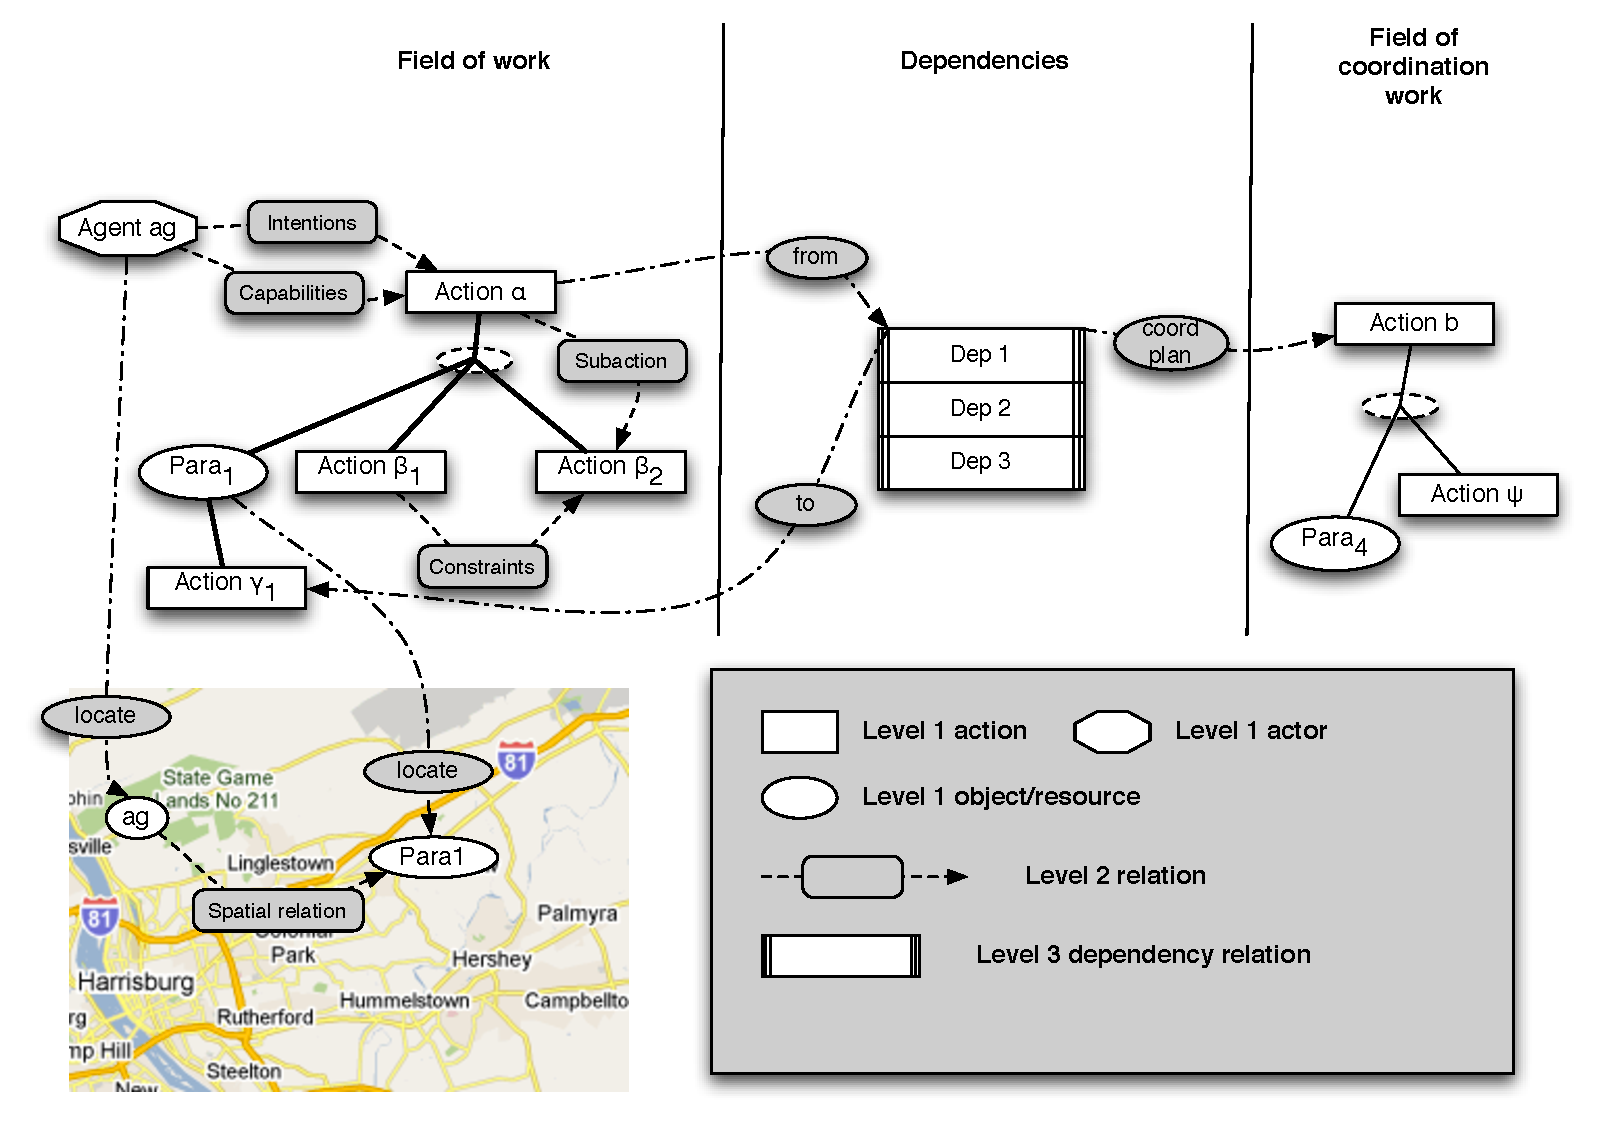
\includegraphics[width=5.5in]{knowledge_repre.pdf} 
   \caption{Representing knowledge with PlanGraph}
   \label{fig:knowledge_repre}
\end{figure}

\subsection{Structure of the PlanGraph}

A PlanGraph is a schematic tree representation of a shared plan about a collaborative activity in a hierarchical way (Figure \ref{fig:plangraph}). The root of a PlanGraph is the overall collaborative activity, which is decomposed recursively as actions through the adoption of recipes. The whole tree therefore is the plan corresponding to the root action, while each sub-tree with a sub-action as the root represents the plan for that sub-action. In a PlanGraph, we also handle the knowledge-preconditions as a special type of node Ð parameters. Nodes with oval shape in Figure \ref{fig:plangraph} indicate parameters, and nodes with rectangle shape represent subplans. A plan underneath a parameter node is the plan for identifying the parameter. 

Unlike the notion of recipe graph (Rgraph) developed by Lochbaum (1998), a PlanGraph not only represents how a complex action is decomposed into sub-actions, but also encodes the mental states of agents towards each action and sub-action. Therefore, each node in the PlanGraph includes several slots to store the participating agents' mental states: (a) Intentions are slots recording the system's beliefs about intentions of each agent towards the action; (b) Capability indicates the systemÕs belief about the ability to perform the action, such as whether they can identify a recipe for the action or whether the agents can bring it about; (c) Beliefs are slots for recording the system's beliefs about what the other agents also believe about.

\begin{figure}[htbp] %  figure placement: here, top, bottom, or page
   \centering
   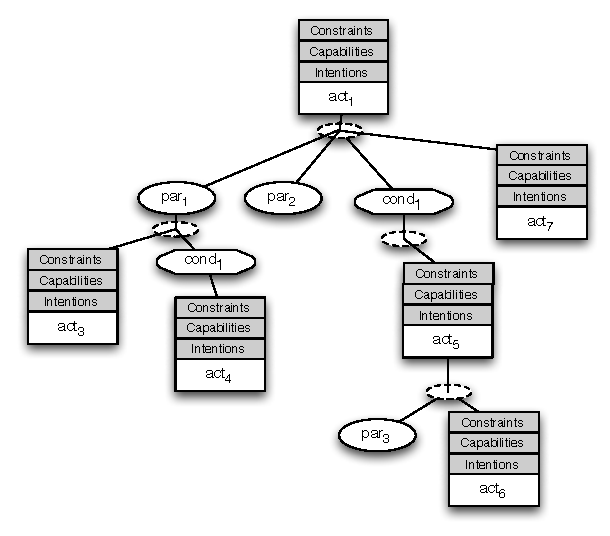
\includegraphics[width=4in]{plangraph.pdf} 
   \caption{Structure of a PlanGraph}
   \label{fig:plangraph}
\end{figure}

Therefore, the development of a collaborative activity can be represented as a dynamic process of constructing a PlanGraph. Before the collaboration begins, the PlanGraph is empty. As agents perform some actions to fulfill the shared goal, new plan nodes are introduced to the PlanGraph. If the root action in the PlanGraph is complex, agents will decompose it by selecting a recipe collaboratively. Then, agents move their attention to the parameters and sub-actions. These sub-actions may themselves be complex, and will become the subjects of further elaboration to form a sub-plan for performing. In the course of development, the PlanGraph will store the mental states of the agents toward each action node and update them in corresponding slots. 

In general, a PlanGraph represents the dynamic knowledge about the underlying collaborative activity. It indicates those beliefs and intentions of the agents that have been established at that point, the actions that have been performed, and the parameters about these actions. 

\subsection{Representing activities} % (fold)
\label{sub:representing_activities}

\subsubsection{Representing basic elements} % (fold)
\label{ssub:representing_basic_elements_of_a_collaborative_activity}
The four basic elements we define in a geo-collaborative activity are: actors, actions, resources, and objects. They can be modeled as the first-class components in a PlanGraph structure. 

\textbf{Actors as agents of plans.}

Actors are represented as agents responsible for a plan/sub-plan and capable of performing actions in the plan. Each agent node in the PlanGraph maintain the current state of the corresponding actor, such as the location, the role of the actor, and the expertise he/she has. Each agent node also includes an cursor that is always attached to an action that is the current focus of the corresponding actor in the whole plan. In addition, each agent node has a unique ID which allows the retrieval of more long-term contextual knowledge (e.g. gender, age, familiarity with the activity involved, ethnicity, etc.) about this particular actor from the knowledge base.

\textbf{Actions as plans/sub-plans}

Actions are modeled within the hierarchical structure of the PlanGraph as plans/sub-plans. The goal of the action is represented as a plan node, including information about various properties, such as the type, the complexity, or the execution status of the action. Furthermore, the selected plan to perform this action can be derived from the subsidiary parameter or action nodes, which can include sub-plans by themselves. 

\textbf{Objects and resources as parameters}

Objects and resources are modeled as parameters in a PlanGraph. They define the knowledge or physical pre-conditions that have to be satisfied prior to an action being performed. Each parameter node records information about the current states of the corresponding object or resource in the domain, such as the location of a rescue vehicle, or the capacity of the decontamination station. Parameter nodes can be collective or individual. A collective parameter indicates an object or resource with multiple values, for instance, the parameter representing all the victims in a rescue operation. An individual parameter represents an instance of an object or resource, such as the rescue vehicle used in a particular delivery task. 

% subsubsection representing_basic_elements_of_a_collaborative_activity (end)
\subsubsection{Representing relations} % (fold)
\label{ssub:representing_relations}
The second level of knowledge in the field of work includes the relations among the basic elements in the activity structure and in the geographic space. They can be modeled as the relations among components in a PlanGraph structure, or inferred from their properties.

\textbf{Relations between actors and their actions}

The relations between actors and their actions are modeled based on the formal specification of mental attitudes requirements of participants in a collaborative activity. The specification is given in terms of beliefs, mutual beliefs, and intentions of the participants. Intentions are used to represent an agent’s commitments to actions. Besides, several belief predicates are also defined to represent the knowledge an agent has about its ability to perform an action. Each action node in a PlanGraph includes several slots to To model these mental attitudes: (a) \emph{Intentions} are slots recording the intentions of each participating actor towards the corresponding action; (b) \emph{Capability} indicates the system’s belief about the ability of each participant to perform this action, such as whether they can identify a recipe or they can bring it about.

\textbf{Relations between actions}

The two major types of relations between actions are composition and precedence. The former is directly encoded in the hierarchical structure of a PlanGraph. Each action node has a slot \emph{subactions} recording its subsidiary actions under current plan. As a result, the fact that acton $a_1$ is included in the \emph{subactions} slot of action $a_2$ represents the relation that action $a_1$ is the subsidiary action of doing $a_2$. The precedence relation that reflects the temporal order of doing two actions is encoded in the \emph{constraints} slot of each action node. In a PlanGraph, each action node also includes a slot \emph{constraints} to recording the system’s beliefs about a set of propositions, each of which represents certain constraint information about the action, e.g. the deadline of doing the action, the actions that need to be performed before the action, etc. The temporal order of two actions can be represented in their respective \emph{constraints}, indicating that the other action must be performed before/after this action.

\textbf{Relations between objects/resources and actions}

The relations between object/resources and actions are modeled as the composition relations between action nodes and parameter nodes in a PlanGraph. Each action node has a slot \emph{parameters} recording all the parameters under current plan, and each parameter has a slot \emph{subactions} recording the current plan to identify or manipulate the parameter. The distinction between objects and resources is relative, depending on their relations to the actions in the PlanGraph. A parameter is an object to the action that is used to identify or manipulate its value, but it is a resource to the action that is at the same level of the parameter and use the parameter during the performance. 

\textbf{Spatial relations}

The spatial relations between basic elements in the field of work are not represented directly in the PlanGraph. Instead, all the basic elements with a geographic dimension in the PlanGraph are geo-referenced as properties. Each actor's current location is stored as an attribute of each agent node. Each parameter, if its values have geographic meaning, such as the location of a rescue vehicle, or the shape of an incident area, are stored with corresponding coordinates in the geographic reference framework. In this way, although the spatial relations among these elements are not directly recorded in the PlanGraph, they can be easily perceived or calculated based on their references in the geographic space. 

% subsubsection representing_relations (end)
% subsection representing_activities (end)

\subsection{Representing local scopes} % (fold)
\label{sub:representing_local_scopes}
\textcolor{red}{To be Added.}

% subsection representing_local_scopes (end)

\subsection{Representing dependencies} % (fold)
\label{sub:representing_dependencies}

According to the SharedPlans theory, the commitment to an action entails different types of obligations to the components of this action's current plan. Based on the SharedPlans theory, we can utilize the following rules to detect basic dependency relations in the activity structure:

\begin{enumerate}
	\item \textbf{Action Performance}: if an agent or a group of agent intend to develop a FSP of collaborative action $a$, then they will also intend to develop a FSP for each subsidiary action:\\
	$Int.Th(ag, a, t) \land b_i\in Recipes(a) \Rightarrow Int.Th(ag, b_i, t)$\\
	This rule can be used to detect the subsidiary dependency relation between two action nodes. The fact that $a_1$ is a subsidiary action node under $a_2$ indicates a dependency of $subsidiary(a_1, a_2)$. 
	
	\item \textbf{Parameter Identification}: the formalization in SharedPlans specifies that all the agents must intend-that the parameters of the group action be identified. If the actors have the intention that they will develop a FSP of collaborative action $a$, then they will also intend that they will develop a FSP to identify each parameter of $a$:\\
	$Int.Th(ag, a, t) \land p_i\in Params(a) \Rightarrow Int.Th(ag, id.Params(p_i), t)$\\
	This rule can be used to detect the dependency relations between an action and a parameter node. $consume(a, r)$ is detected when a parameter node representing a resource $r$ and an action node $a$ are siblings; $producer(a, r)$ can be extracted from the fact that $a$ is a subsidiary action node under the parameter node representing a resource $r$. 
	
	\item \textbf{Actor Commitment}: In order to develop a FSP of an collaborative action $a$, at least one of the actors need to commit to the action and has the capability to perform it:\\
	$FSP(a, a_t) \land ag\in Agents(a) \Rightarrow Int.Th(ag, a, a_t) \land CBA(ag, a, a_t)$\\
	This rule can be used to detect the dependency relations between an action and an agent. $commit(ag,a)$ relation between an agent and an action is encoded in the \emph{Intentions} slot attached to each action node, and $capable(ag, a)$ is encoded in the \emph{Capability} slot attached to each action node.
	
	\item \textbf{Constraint Satisfaction}: it requires that all the members of the group be committed to making sure that the constraints for doing action $a$ will hold:\\
	$Int.Th(ag, a, a_t) \Rightarrow Int.Th(ag, constr(a), a_t)$\\
	This rule can be used to detect the dependency relations that are encoded in the \emph{constraints} slot of each plan node. For example, if the one of the constraints of performing action $a_1$ indicates that $a_2$ must be performed at a time before $a_1$, then the dependency relation of $precede(a_2, a_1)$ can be detected.
\end{enumerate}

% subsection dependency_relations_in_the_activity_structure (end)
Table~\ref{tab:basic_deps_pg} indicates the basic dependency relations that can be detected based on these rules. 

%\begin{table}[htdp]
\begin{center}
\begin{longtable}{|p{4.5cm}|p{8.5cm}|}
\hline
Dependency & Structure in PlanGraph\\
\hline
$subsidiary(a_1, a_2)$ &  $a_1$ is a subsidiary plan node under $a_2$: \par 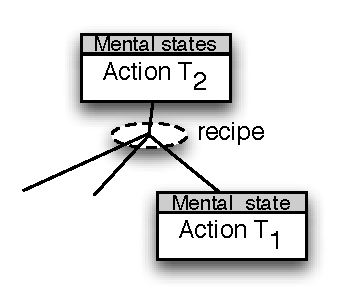
\includegraphics[scale=0.6]{subsidiary.pdf}\\
\hline
$precede(a_1, a_2)$ &  $a_1$ and $a_2$ as ordered siblings: \par 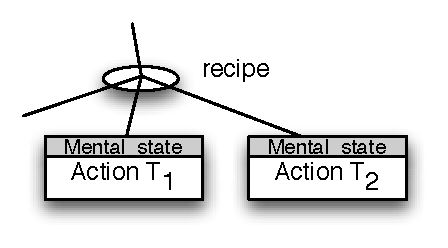
\includegraphics[scale=0.6]{precede.pdf}\\
\hline
$commit(ag,a)$ & the \emph{Intentions} slot attached to each plan node: \par 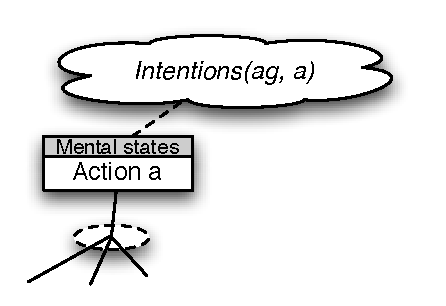
\includegraphics[scale=0.6]{commit.pdf}\\
\hline
$consume(a, r)$ & a parameter node representing a resource $r$ and  a plan node $T$ as siblings: \par 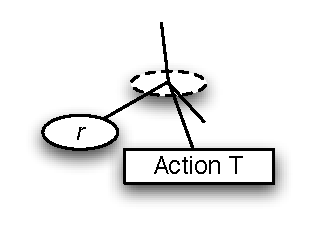
\includegraphics[scale=0.6]{use.pdf}\\
\hline
$produce(a, r)$ &  $a$ is a subsidiary action node under the parameter node representing a resource $r$: \par 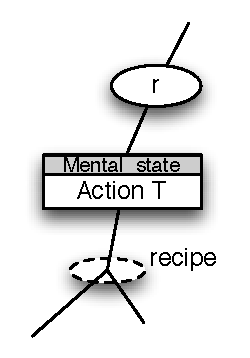
\includegraphics[scale=0.6]{generate.pdf}\\
\hline
\caption{Identifying basic dependencies in PlanGraph}
\label{tab:basic_deps_pg}
\end{longtable}
\end{center}
%\end{table}%

\section{Construction and Development of the Model} % (fold)
\label{sec:construction_and_development_of_the_model}
\subsection{The Development of PlanGraph} % (fold)
\label{sub:the_development_of_plangraph}
Considering the collaborative activity as a process from a partial SharedPlan to a full SharedPlan among the participants, the PlanGraph, which is used to represent the collaborative activity, should also be considered as dynamically developed. To facilitate the development of PlanGraph, the PlanGraph model provides the reasoning mechanisms to decide how the interaction between the system and human participants, or between the human participants, influences the state of collaborative activity and update the changes in the PlanGraph. In general, the reasoning mechanism in PlanGraph model includes two steps: the plan explanation and the plan elaboration.

\subsubsection*{Plan Explanation}
Participants in a collaborative activity need to interact with each other to contribute to the activity. It is through the communication between the participants that collaboration can be enacted. Therefore, the input of an agent can be treated as the way that the agent tries to express their intentions to the other agents in the collaborative activity. Plan explanation is the step where the system attempts to explain how the meanings of the new piece of interaction relate to the current PlanGraph. In general, the new input is said to be meaningfully merged with the current collaboration context if one of the following conditions is satisfied:

\begin{enumerate}
\item The new input provides a piece of information that helps the agents to assign/change a value to a parameter in the current PlanGraph. 
\item The new input provides more details on the performance of a complex action in the PlanGraph. For example, the user suggests performing a sub-action or identifying a parameter in order to complete the action.
\item The new input helps to establishing necessary mental states for a collaborative action. In this case, the agent's new input serves as an indicator of the speaker's mental attitudes, such as confirmation or refusal towards certain states of fairs. 
\end{enumerate}

If the new user input can be successfully explained in current PlanGraph, it will be merged to update the PlanGraph accordingly, i.e. the contextual information about the ongoing activity is changed.

\subsubsection*{Plan Elaboration}
The main goal in elaboration stage is to advance the collaborative activity from the system side based on the change from the new input. After the interpretation process, the context of the activity is changed. Therefore, the system needs to elaborate the PlanGraph to accommodate the changes. The elaboration process begins with the root node of the PlanGraph and uses the depth-first traverse to visit the whole plan based on reasoning rules associated with PlanGraph model. The elaboration ends when no more parts of the PlanGraph can be further elaborated.

The system can elaborate the PlanGraph in several ways. First, the system can contribute to the collaborative activity by retrieving a recipe for an action from the knowledge base. Second, the system can execute the basic actions that can be performed without further inputs from other human agents. Lastly, the system can identify the value for a parameter by retrieving the default or suggested values from the knowledge base. 

After the elaboration process, the PlanGraph again reflects the current state of the collaborative activity. Therefore, the information from the PlanGraph can be used by the system to represent the current state of the activity context. 

This elaboration process also attempts to discover all the open nodes in the PlanGraph that might be addressed later in the collaboration, such as unidentified parameters, unperformed actions, conflicting beliefs, missing details, or ambiguous choices. These possible open nodes are   stored in an agenda to include all the possible attentional states that require further development in the collaboration. During the elaboration process, when the system encounters some problem to elaborate an action node, is unable to identify the value of a parameter, or fail to execute an action, the system will put the node into the agenda.
% subsection the_development_of_plangraph (end) 

% section construction_and_development_of_the_model (end)

% chapter field_of_work (end)




 

